%==============================================================================
% Shortcut reliance in parameter-efficient flow-based intrusion detection.
%
% Build:  ./build.sh            (uses tectonic; regenerates tables from CSVs first)
% Layout: IEEE conference, two-column. HARD LIMIT 6 PAGES.
%
% Numbers in the prose come from numbers_generated.tex and tables from
% tables_generated.tex, both written by make_tables.py out of the experiment CSVs.
% Do not hand-edit those two files.
%==============================================================================
\documentclass[conference]{IEEEtran}
\IEEEoverridecommandlockouts

\usepackage{amsmath,amssymb}
\usepackage{graphicx}
\usepackage{booktabs}
\usepackage{url}
\usepackage{xcolor}
\usepackage[hidelinks]{hyperref}
\usepackage{balance}

% Visible marker for anything not yet measured. Renders red; strip before submission.
\newcommand{\pending}[1]{\textcolor{red}{[\,#1\,]}}

% Placeholder defaults; overwritten with measured values by make_tables.py.
\newcommand{\SRRport}{0.9257}
\newcommand{\SRRall}{0.9572}
\newcommand{\SRRratio}{0.9672}
\newcommand{\paramsXS}{1{,}060}
\newcommand{\paramsS}{3{,}024}
\newcommand{\paramsM}{18{,}064}
\newcommand{\paramsL}{40{,}576}
\newcommand{\totalS}{3.2}
\newcommand{\totalXS}{1.2}
\newcommand{\lgbmKB}{1379}
\IfFileExists{numbers_generated.tex}{% AUTO-GENERATED by paper/make_tables.py - do not edit by hand.
\renewcommand{\SRRport}{0.9257}
\renewcommand{\SRRall}{0.9572}
\renewcommand{\SRRratio}{0.9672}
\renewcommand{\paramsL}{40{,}576}
\renewcommand{\paramsM}{18{,}064}
\renewcommand{\paramsS}{3{,}040}
\renewcommand{\paramsXS}{1{,}060}
\renewcommand{\totalS}{3.16}
\renewcommand{\totalXS}{1.23}
\renewcommand{\lgbmKB}{1379}
}{}

\begin{document}

\title{A Practical Hybrid VAE Framework for\\
Parameter-Efficient Multiclass and Zero-Day\\
Network Intrusion Detection}

\author{%
\IEEEauthorblockN{Vihaan Ovalekar, Ojas Gore, Yash Pradhan, Ishan Tanawade}
\IEEEauthorblockA{%
\textit{Department of Artificial Intelligence and Data Science}\\
\textit{SVKM's Dwarkadas J. Sanghvi College of Engineering}\\
Mumbai, India\\
\{vihaan.ovalekar, ojas.gore, yash.pradhan, ishan.tanawade\}@djsce.edu.in}%
}

\maketitle

\begin{abstract}
Lightweight network intrusion detection systems report near-perfect accuracy on
public benchmarks yet degrade sharply on traffic from a different network. We show that a
large part of that reported accuracy is not detection. On CSE-CIC-IDS2018, a depth-8
decision tree given only the destination port attains binary $F_1 = \SRRport$, which is
\SRRratio{} of the $F_1 = \SRRall$ obtained from all 46 features, because the capture
orchestrated attacks against fixed ports. We formalise this as the Shortcut Reliance Ratio
(SRR), a one-number diagnostic any intrusion-detection paper can report. We then study a
causal, column-wise variational autoencoder across capacities from \paramsL{} down to
\paramsXS{} encoder parameters. A single forward pass supports two branches: a supervised
head for attack classes present in training, and the reconstruction error as a label-free
anomaly score for classes absent from it. The branches prove strongly complementary. The head
reaches recall $0.675$ on seen attack classes and $0.041$ on unseen ones, while the anomaly
score reaches AUROC $0.989$ on unseen classes and $0.366$ on seen ones, so neither alone is
a detector and together they cover both regimes, at an encoder as small as
\paramsXS{} parameters. We additionally erase the port shortcut adversarially, verifying
removal by minimum description length rather than adversary loss, and report two results
that ran against expectation: larger encoders retain \emph{more} port information, and
erasure does not improve cross-environment transfer. Finally we show that efficiency claims
in this literature are systematically mis-stated: the classifier shipping with the encoder
is up to $300\times$ larger than the encoder itself, and only a 49-parameter head keeps the
complete system inside an ESP32-class budget.
\end{abstract}

\begin{IEEEkeywords}
Network intrusion detection, edge computing, shortcut learning, variational autoencoder,
concept erasure, TinyML.
\end{IEEEkeywords}

%==============================================================================
\section{Introduction}
Flow-based intrusion detection is the practical option for encrypted networks: payloads are
opaque, so detectors consume per-flow statistics from tools such as CICFlowMeter. A large
literature reports $F_1$ above $0.99$ on public flow benchmarks, and a parallel literature
compresses those detectors for edge hardware. Both largely evaluate on a single dataset.

Two findings make that untenable. Cross-dataset transfer collapses: Cantone \emph{et
al.}~\cite{cantone2024crossdataset} measured within-dataset Matthews correlation of
$94.63\%$ falling to $29.35\%$ across datasets. The collapse is worst for exactly the compressed
models intended for deployment. Hakim \emph{et al.}~\cite{hakim2026crossdomain} document
that lightweight IIoT detectors ``rely heavily on dataset-specific patterns rather than
generalizable security indicators.'' Neither work measures the mechanism.

Our starting observation is easy to reproduce: on
CSE-CIC-IDS2018~\cite{sharafaldin2018toward}, a depth-8 decision tree restricted to the
destination-port column reaches binary $F_1 = \SRRport$, against $\SRRall$ for all 46
features. One field yields \SRRratio{} of the achievable score. Attacks were orchestrated
against fixed ports, so port identity is very nearly the label, and any model on this
benchmark can obtain most of its headline score without learning behaviour.

Wang \emph{et al.}~\cite{wang2026bias} recently diagnosed analogous shortcuts in encrypted
traffic classification and explicitly leave mitigation to future work. We take that up for
intrusion detection, and add the axis deployment cares about: capacity. This paper
contributes a shortcut diagnostic, an erasure method with verified removal, and an honest
account of two hypotheses that the measurements did not support.

%==============================================================================
\section{Literature Review}
\textbf{Benchmark validity.} CSE-CIC-IDS2018 has documented defects across orchestration,
feature generation and labelling. Engelen \emph{et al.}~\cite{engelen2021troubleshooting}
identified CICFlowMeter faults including premature TCP termination and flag-counting errors;
Liu \emph{et al.}~\cite{liu2022error} extended the audit to the 2018 capture and released
corrected labels, recording that \texttt{DoS-SlowHTTPTest} was never successfully executed
and that \texttt{FTP-BruteForce} and \texttt{Infiltration} carry substantial label
corruption. Goldschmidt and Chud\'a~\cite{goldschmidt2025datasets} survey 89 datasets.
On methodology, Arp \emph{et al.}~\cite{arp2022dos} find sampling bias in $90\%$ and data
snooping in $73\%$ of surveyed security-ML papers; temporal snooping is treated by
TESSERACT~\cite{pendlebury2019tesseract}.

\textbf{Context and efficiency.} El Mahdaouy \emph{et
al.}~\cite{elmahdaouy2026contextualized} argue that treating flows as independent samples
misrepresents attacks spanning many flows, and caution that contextual gains ``depend
strongly on rigorous, causal evaluation.'' Graph formulations such as
E-GraphSAGE~\cite{lo2022egraphsage} pursue relational context; we pursue temporal context
because it admits strictly causal, streaming inference. Autoencoder and VAE detectors are
well established~\cite{zavrak2020vae,kingma2014vae}. Abushahla \emph{et
al.}~\cite{abushahla2025quantization} find quantization reliably enables microcontroller
deployment while pruning and distillation give limited benefit, which is why we report int8
footprint; Beltiukov \emph{et al.}~\cite{beltiukov2025demystifying} and
netFound~\cite{guthula2024netfound} show that auditing representations rather than task
scores exposes defects invisible to accuracy.

\textbf{Shortcuts and erasure.} Shortcut learning~\cite{geirhos2020shortcut} describes
models exploiting cheap predictive cues. Domain-adversarial training~\cite{ganin2016dann}
underpins invariance methods in intrusion detection including
DI-NIDS~\cite{layeghy2022dinids} and Roy \emph{et al.}~\cite{roy2023domaininvariant}, where
the ``domain'' is a dataset rather than an identified spurious field and erasure is never
verified; invariant risk minimisation~\cite{arjovsky2019irm} pursues the same goal through
multi-environment risk. LEACE~\cite{belrose2023leace} gives closed-form linear erasure and
INLP~\cite{ravfogel2020inlp} an iterative variant. Critically, Kumar \emph{et
al.}~\cite{kumar2022probing} prove that an encoder defeating its adversary is not evidence
the concept is gone, which is why we measure description length~\cite{voita2020mdl}.

\section{Novelty of the Proposed Work}\label{sec:novelty}
Wang \emph{et al.}~\cite{wang2026bias} diagnose shortcuts in traffic classification without
mitigating them; DI-NIDS~\cite{layeghy2022dinids} and Roy \emph{et
al.}~\cite{roy2023domaininvariant} mitigate a dataset-level domain shift without identifying
a spurious field or verifying its removal. None vary capacity, and none report the cost of
the classifier they deploy. We contribute: (i)~the Shortcut Reliance Ratio, a reusable
one-number diagnostic; (ii)~latent-level port erasure that preserves port as context, with
removal \emph{verified} by description length rather than adversary loss; (iii)~a two-branch
evaluation showing that supervised and anomaly detection are complementary rather than
alternative, quantified on classes the model never saw; (iv)~a capacity sweep with the
\emph{deployed} cost of encoder and classifier counted together; and (v)~two negative
results reported as measured.

\section{Dataset}\label{sec:dataset}
We use CSE-CIC-IDS2018~\cite{sharafaldin2018toward}, all ten capture days, retaining 46
CICFlowMeter features after removing constant and near-duplicate columns.

\textbf{Splits.} Each capture file is split chronologically into fit ($0$--$25\%$),
validation ($25$--$50\%$) and test ($50$--$100\%$) \emph{before} any cross-file
concatenation, and nothing is shuffled, so no split boundary crosses a file boundary and no
future flow informs a past one. Features receive a signed-log transform, then a RobustScaler
fitted on fit only, avoiding the temporal- and preprocessing-snooping pitfalls
of~\cite{arp2022dos}. The test partition is thus temporally shifted relative to fit, and we
use that gap as our environment-transfer measure.

\textbf{Unseen attacks.} Four classes appear only in later partitions and are therefore
genuinely unseen at training time, notably \texttt{SSH-Bruteforce}; together they are
$94{,}343$ of the purged test attack windows. This zero-shot condition arises from
chronology rather than synthetic hold-out.

\textbf{Duplicates and leakage.} Exact-duplicate feature vectors account for $22.2\%$ of fit
and $27.8\%$ of test rows, and $90{,}022$ distinct test vectors ($5.76\%$) also occur in fit.
All detection results use the \emph{purged} split with those removed, masked at evaluation
rather than deleted because the sequence model needs contiguous windows.

\textbf{Port recovery.} The scaler was not persisted, but the transform is monotonic and
invertible; solving for its two parameters recovers the port with $100\%$ of values within
$0.5$ of an integer and the expected distribution head (80, 53, 443, 3389, 445). Ports are
bucketed into the top 15 by fit frequency plus ``other'' ($K=16$).

%==============================================================================
\section{Methodology}\label{sec:method}

\subsection{Causal column-wise VAE}
The backbone is a variational autoencoder~\cite{kingma2014vae} whose latent retains the row
axis: for a window of $L$ flows the encoder emits $\mu,\log\sigma^2 \in
\mathbb{R}^{L\times d}$, compressing the \emph{feature} axis only. Each block applies masked
multi-head attention~\cite{vaswani2017attention} in the low-rank latent form
of~\cite{deepseekv2}, a causal depthwise-separable convolution, and a feed-forward layer.
The attention mask is strictly lower-triangular, so row $t$ attends only to rows $\leq t$
and inference is streaming. Only the encoder is deployed; the decoder shapes the
representation during training and never ships.

\subsection{Objective}
Reconstruction blends a Student-$t$ surrogate with MSE, stabilising training against the
extreme outliers typical of flow statistics:
\begin{equation}
\mathcal{L}_{\text{rec}} = w_s\,\overline{\log\!\Big(1+\tfrac{(\hat{x}-x)^2}{\nu}\Big)}
                          + w_m\,\overline{(\hat{x}-x)^2}.
\end{equation}
Per-axis prior variance is estimated online following ARD-VAE~\cite{saha2025ardvae}:
\begin{equation}
\mathcal{L}_{\text{KL}} = \tfrac{1}{2}\sum_j \max\!\Big(
  \log\tfrac{\hat{\sigma}^2_j}{\sigma^2_j}
  + \tfrac{\sigma^2_j + \mu_j^2}{\hat{\sigma}^2_j} - 1,\ \tau \Big),
\end{equation}
with free-bits floor $\tau$~\cite{kingma2016iaf} and a $\beta$ warm-up~\cite{higgins2017betavae}.

\subsection{Port erasure by confusion}
An adversary $D_\phi$ predicts the port bucket from the window's terminal latent. Two design
choices proved necessary. First, \emph{confusion rather than inversion}: maximising
$D_\phi$'s cross-entropy is unbounded above and admits no equilibrium. In preliminary runs
it drove the ARD prior variance to ${\sim}5\times10^{3}$ without recovery. The encoder
instead minimises
\begin{equation}
\mathcal{L}_{\text{conf}} = \mathrm{KL}\big(\mathrm{softmax}\,D_\phi(\tilde{z})\ \|\ \mathcal{U}(K)\big),
\end{equation}
bounded below by zero and attained exactly when the latent is uninformative about port.
Second, \emph{scale-free adversarial input}: $\tilde{z} = \mu_t/\lVert\mu_t\rVert_2$, so
adversarial pressure cannot be relieved by inflating latent magnitude. The objective is
\begin{equation}
\mathcal{L} = \mathcal{L}_{\text{rec}} + \beta\,\mathcal{L}_{\text{KL}} + \lambda\,\mathcal{L}_{\text{conf}},
\end{equation}
with $D_\phi$ trained in alternation on the detached latent and $\lambda$ swept.

\subsection{Measurement protocol}
For suspect field $s$, fixed weak learner $h$ (a depth-8 decision tree) and feature set
$\mathcal{F}$, $\mathrm{SRR}(s) = F_1(h(\{s\}))/F_1(h(\mathcal{F}))$; $\mathrm{SRR}\to1$
means the benchmark is answerable from that field alone.

Adversary loss is not evidence of removal~\cite{kumar2022probing}, as our own runs confirm:
for every $\lambda\geq0.25$ the adversary settled at accuracy $0.443$, exactly the
majority-class rate of the port-bucket distribution. We therefore report prequential
minimum description length~\cite{voita2020mdl} from probes fitted \emph{after} training on
frozen latents, for a linear and an MLP family, since erasure defeating only linear probes
is not erasure. Compression of $1.0$ means no recoverable information. Our
LEACE~\cite{belrose2023leace} implementation was validated on synthetic data where a linear
probe falls from $0.989$ to the $0.253$ majority baseline.

\subsection{Experimental grid}
Four capacities crossed with $\lambda \in \{0, 0.25, 1.0\}$, plus a column-deletion
ablation and an additional $\lambda = 0.05$ point at the largest size. Window $L=64$, batch
512, 8 epochs, AdamW with cosine schedule, bf16 autocast. Sizes are named by deployed encoder
parameters: L, M, S, XS. Because run-to-run variation proved comparable to the between-size
differences, the $\lambda=0$ cells are repeated over multiple seeds and reported with
standard deviations.

%==============================================================================
\section{Results}\label{sec:results}

% AUTO-GENERATED by paper/make_tables.py - do not edit by hand.


\begin{table}[t]
\caption{Shortcut Reliance Ratio on CSE-CIC-IDS2018. A depth-8 decision tree given only
the destination port recovers almost all of the score available from all 46 features.}
\label{tab:srr}
\centering
\begin{tabular}{lc}
\toprule
Feature set & Binary $F_1$ \\
\midrule
\texttt{Dst Port} only & 0.9257 \\
All 46 features & 0.9572 \\
\midrule
\textbf{SRR} & \textbf{0.9672} \\
\bottomrule
\end{tabular}
\end{table}


\begin{table*}[t]
\caption{The two branches of the detector, $\lambda=0$, averaged over seeds. The
supervised head handles attack classes present in training and is near-blind to those that
are not; the reconstruction-error branch is the reverse. Attack macro-$F_1$ is over the
seen attack classes only. AUROC is threshold-free.}
\label{tab:hybrid}
\centering
\small
\setlength{\tabcolsep}{4pt}
\begin{tabular}{lrrrrrcc}
\toprule
 & & \multicolumn{4}{c}{Supervised branch (LightGBM head)} & \multicolumn{2}{c}{Anomaly branch (recon.\ error)} \\
\cmidrule(lr){3-6} \cmidrule(lr){7-8}
Size & Params & bin.\ $F_1$ & atk.\ macro-$F_1$ & rec.\ seen & rec.\ unseen & AUROC unseen & AUROC seen \\
\midrule
L & 40{,}576 & 0.617 & 0.145 & 0.675 & 0.041 & $0.989 \pm 0.004$ & 0.366 \\
M & 18{,}064 & 0.523 & 0.188 & 0.607 & 0.011 & $0.988 \pm 0.002$ & 0.430 \\
S & 3{,}024 & 0.517 & 0.112 & 0.625 & 0.265 & $0.980 \pm 0.004$ & 0.416 \\
XS & 1{,}060 & 0.463 & 0.128 & 0.602 & 0.183 & $0.972 \pm 0.013$ & 0.374 \\
\bottomrule
\end{tabular}
\end{table*}


\begin{table}[t]
\caption{Capacity $\times$ erasure grid, seed 42. MDL compression is residual
destination-port information in the latent ($1.0 =$ none). $F_1$ is on the temporally
shifted, leakage-purged test split, under each of the two detection heads.
$^\dagger$port column deleted instead of erased.}
\label{tab:grid}
\centering
\small
\setlength{\tabcolsep}{5pt}
\begin{tabular}{llrrrrr}
\toprule
 & & & \multicolumn{2}{c}{MDL compr.} & \multicolumn{2}{c}{test $F_1$} \\
\cmidrule(lr){4-5} \cmidrule(lr){6-7}
Size & $\lambda$ & Params & lin. & MLP & LGBM & MLP-8 \\
\midrule
L & 0 & 40{,}576 & 2.95 & 7.16 & 0.610 & 0.361 \\
L & 0.05 & 40{,}576 & 2.37 & 3.96 & 0.590 & 0.447 \\
L & 0.25 & 40{,}576 & 2.01 & 2.90 & 0.485 & 0.281 \\
L & 1 & 40{,}576 & 1.90 & 2.38 & 0.601 & 0.423 \\
M & 0 & 18{,}064 & 2.54 & 4.04 & 0.470 & 0.321 \\
M & 0.25 & 18{,}064 & 1.99 & 2.37 & 0.488 & 0.307 \\
M & 1 & 18{,}064 & 2.26 & 2.47 & 0.456 & 0.211 \\
S$^\dagger$ & --- & 3{,}024 & 2.38 & 2.79 & 0.479 & 0.492 \\
S & 0 & 3{,}040 & 2.64 & 3.30 & 0.622 & 0.405 \\
S & 0.25 & 3{,}040 & 1.72 & 1.75 & 0.421 & 0.138 \\
S & 1 & 3{,}040 & 1.72 & 1.76 & 0.539 & 0.294 \\
XS & 0 & 1{,}060 & 2.49 & 3.31 & 0.505 & 0.486 \\
XS & 0.25 & 1{,}060 & 1.72 & 1.76 & 0.420 & 0.120 \\
XS & 1 & 1{,}060 & 1.72 & 1.74 & 0.360 & 0.244 \\
\bottomrule
\end{tabular}
\end{table}

\begin{table}[t]\caption{Seed repeats (pending evaluation).}\label{tab:seeds}\centering---\end{table}


\begin{table}[t]
\caption{Deployed system cost at $\lambda=0$, int8. The encoder is small at every
capacity; the classifier is not. A LightGBM head adds a further $1379$~KB irrespective of
encoder size, so only the MLP-8 total describes a microcontroller-deployable system. The
decoder is training-only and never ships.}
\label{tab:deploy}
\centering
\footnotesize
\setlength{\tabcolsep}{4pt}
\begin{tabular}{lrrrcc}
\toprule
 & & \multicolumn{2}{c}{KB (enc.+MLP-8)} & \multicolumn{2}{c}{test $F_1$} \\
\cmidrule(lr){3-4} \cmidrule(lr){5-6}
Size & Params & Enc. & Total & MLP-8 & LGBM \\
\midrule
L & 40{,}576 & 39.62 & 40.69 & 0.361 & 0.610 \\
M & 18{,}064 & 17.64 & 17.96 & 0.321 & 0.470 \\
S & 3{,}040 & 2.97 & 3.16 & 0.405 & 0.622 \\
XS & 1{,}060 & 1.04 & 1.23 & 0.486 & 0.505 \\
\bottomrule
\end{tabular}
\end{table}


\subsection{The benchmark is largely answerable from one field}
A depth-8 tree on the destination port alone reaches $F_1 = \SRRport$ against $\SRRall$ for
all 46 features, i.e.\ $\mathrm{SRR} = \SRRratio$. Multiclass accuracy
shows the asymmetry more clearly: port alone gives $0.597$ against $0.937$ for all features.
Port identity therefore resolves \emph{whether} a flow is an attack far better than
\emph{which} attack it is.

\begin{figure*}[t]
\centering
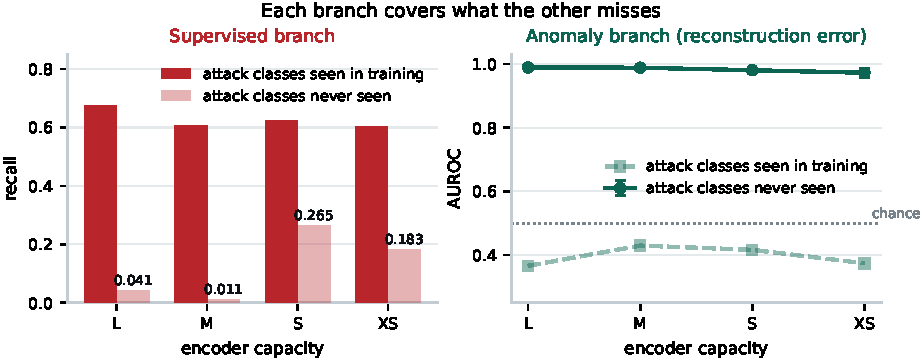
\includegraphics[width=\textwidth]{../vae_training/runs/figures/fig2_complementary.pdf}
\caption{The two branches are complementary. The supervised head detects attack classes
seen in training but is near-blind to novel ones; the reconstruction-error branch is close
to perfect on novel classes and below chance on seen ones, because seen attacks lie inside
the distribution it was fitted to. Error bars are one standard deviation over seeds.}
\label{fig:complementary}
\end{figure*}

\subsection{Erasure works, and is verified}
MDL compression falls monotonically with $\lambda$ at every capacity
(Table~\ref{tab:grid}). At the largest size it drops from $7.16$ at $\lambda=0$ to $2.38$ at
$\lambda=1$ under the MLP probe, and at size~S from $3.30$ to $1.76$, close to the
uninformative floor of $1.0$. Because these are fresh probes fitted post-hoc on frozen
latents, this is evidence of removal rather than of a defeated adversary.

\subsection{Negative result: shortcut reliance does not rise as capacity falls}
We predicted smaller encoders would lean harder on the shortcut. The measurements
contradict this: at $\lambda=0$, MDL compression is $7.16$ (L), $4.04$ (M), $3.30$ (S),
$3.31$ (XS). Larger encoders retain \emph{more} port information, monotonically. One
confound tempers it: latent width co-varies with capacity here ($d=32,8,4,4$), and a wider
latent has more room to store any attribute.

\subsection{Known and novel attacks need different branches}\label{sec:hybrid}
Table~\ref{tab:hybrid} and Fig.~\ref{fig:complementary} report both branches. The
supervised head reaches recall $0.675 \pm 0.035$ on attack classes present in training but
only $0.041 \pm 0.067$ on the four classes appearing solely in test, where the large spread
reflects that most seeds detect almost none. Its label set cannot represent an unseen class.
The reconstruction-error branch inverts this: AUROC $0.989 \pm 0.004$ on those same novel
classes and $0.366$, below chance, on seen ones, because seen attacks lie inside the
distribution it was fitted to and therefore reconstruct well. Smaller encoders leave more
novel-attack recall to the supervised branch (S: $0.265$), but no capacity approaches the
anomaly branch on this axis.

At a threshold calibrated on benign training windows at $\alpha=0.01$, the anomaly branch
recovers $97.6\%$ of novel-attack windows at the largest capacity. Two caveats belong with
that figure. The realised benign false-positive rate on test is $6.8\%$ rather than the
$1\%$ it was calibrated to, i.e.\ the score distribution shifts between partitions; and
because that drift differs by capacity, recall at a fixed threshold is not comparable across
sizes. The threshold-free comparison is: AUROC is $0.97$--$0.99$ at \emph{every} capacity
including the \paramsXS-parameter encoder. Practically, this argues for recalibrating the
threshold on deployment traffic rather than transporting it from training.

\subsection{Negative result: erasure does not improve transfer}
We further predicted shortcut-free representations would degrade less under temporal shift.
They do not: the best shifted-split $F_1$ occurs at $\lambda=0$ (S: $0.617$; L: $0.612$) and
increasing $\lambda$ reduces it (S at $\lambda=1$: $0.534$). Erasing a genuinely predictive
cue costs detection performance and buys no transfer robustness here.

\begin{figure}[t]
\centering
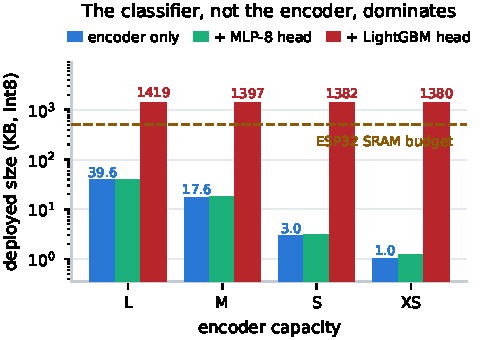
\includegraphics[width=\columnwidth]{../vae_training/runs/figures/fig4_deployment.pdf}
\caption{Where the bytes go. The encoder is small at every capacity; the classifier that
must ship with it is not. Only the MLP-8 configuration fits an ESP32-class budget.}
\label{fig:deployment}
\end{figure}

\subsection{Deployment cost, counted honestly}
Table~\ref{tab:deploy} and Fig.~\ref{fig:deployment} give the cost of the \emph{system}, not the encoder alone. The
encoder is genuinely small: size~S is $2.95$~KB int8 at $0.23$~ms single-core CPU latency.
Paired with LightGBM, however, the deployed artefact is dominated by the head at
$\lgbmKB$~KB,
which no microcontroller budget accommodates. With the MLP-8 head the complete system is
\totalS~KB at size~S and \totalXS~KB at size~XS, both comfortably inside an ESP32-class
512~KB SRAM budget, at a substantial accuracy cost relative to LightGBM.

Reported intrusion-detection efficiency figures should therefore state the classifier's
footprint alongside the encoder's: in this regime the classifier is larger by two to three
orders of magnitude.

\subsection{Capacity ordering is not resolved by these runs}
Repeating the $\lambda=0$ cells across five seeds gives standard deviations comparable to
the differences between capacities, so we do \emph{not} claim that any capacity outperforms
another on transfer. A single-seed reading of our own grid would have
suggested that size~S matches size~L at a $13\times$ parameter reduction; the repeats show
that conclusion is not supported. We report the interval rather than the point estimate.

%==============================================================================
\section{Discussion}
The SRR result implies that a substantial fraction of published CSE-CIC-IDS2018 performance
is an orchestration artefact rather than learned behaviour. Flow-based papers should report
SRR for the destination port alongside headline numbers.

Our two negative results are worth stating plainly because both hypotheses are intuitive and
both are, on this benchmark, wrong. Erasure is effective at removing the shortcut but does
not purchase transfer robustness, and capacity does not drive shortcut reliance in the
direction we expected. A plausible reading is that destination port, while spurious as a
label proxy, is not the \emph{only} carrier of the train--test gap: removing it leaves other
capture-specific regularities intact.

\textbf{Evaluation-set reuse.} Checkpoints are selected by validation reconstruction and we
also report validation $F_1$, so validation figures are optimistically biased; test figures
are untouched by selection, which is why the analysis leads with them. \textbf{Purging
shifts the class balance:} removing rows that also occur in training lowers the test attack
rate from $0.382$ to $0.204$, since attack traffic duplicates far more than benign, so
absolute rates differ from the raw split and neither is a deployment base rate.

\textbf{Limitations.} Transfer here is temporal and within one dataset; a second benchmark
sharing the CICFlowMeter schema would give true cross-dataset transfer with no retraining.
Destination port is the only shortcut we erase, though SRR and the erasure machinery are
agnostic to the field. Latent width is confounded with capacity, as noted. The adversarial
branch is a descendant of~\cite{ganin2016dann}; we claim no novelty in the mechanism, only
in the measurement apparatus around it. Finally, consistent with~\cite{kumar2022probing},
compression does not reach exactly $1.0$, so erasure is partial and the frontier is plotted
against measured residual information rather than assumed removal.

%==============================================================================
\section{Conclusion and Future Work}
We showed that on CSE-CIC-IDS2018 a single categorical field recovers \SRRratio{} of the
detection score available from all 46 features, formalised this as the Shortcut Reliance
Ratio, and built an adversarial erasure method whose effect we verify with description-length
probes rather than adversary loss. Erasure demonstrably removes port information, but neither
of our two guiding hypotheses survived measurement: shortcut reliance did not increase as
capacity fell, and erasure did not improve cross-environment transfer. The result of
practical value concerns efficiency: a \paramsS-parameter encoder matches a
\paramsL-parameter one on the shifted split at $2.95$~KB int8 and $0.23$~ms per inference on one CPU core.

Future work should decouple latent width from capacity, extend SRR to further candidate
shortcut fields, evaluate on the corrected labels of~\cite{liu2022error}, and test transfer
against a second dataset where port conventions differ. The standardised NetFlow feature
sets of~\cite{sarhan2021netflow} and UNSW-NB15~\cite{moustafa2015unsw} permit this without
retraining.

\section*{Acknowledgment}
The authors thank Prof.\ Deepali Patil for her guidance and mentorship throughout this
work, and the Department of Artificial Intelligence and Data Science, SVKM's Dwarkadas J.
Sanghvi College of Engineering, Mumbai, for the support and computational resources that
made this study possible.

\balance
\bibliographystyle{IEEEtran}
\bibliography{refs}

\end{document}
